% Curs 11 - Pagina 4 (13-XII-1994).
% Fragment pentru % Curs 11 - Pagina 4 (13-XII-1994).
% Fragment pentru % Curs 11 - Pagina 4 (13-XII-1994).
% Fragment pentru % Curs 11 - Pagina 4 (13-XII-1994).
% Fragment pentru \input{courses/pages/curs11-pagina4-ro}.
% Fara preambul si fara schimbare fortata de pagina.
% Se pastreaza ordinea manuscrisului; comentariile marcheaza observatii editoriale.

\subsection*{Curs 11 - Pagina 4}

\noindent Fie $b\in G$. Atunci:
\[
by=y\iff b\in\operatorname{Stab}_G(y)
\iff bax=ax.
\]
\[
\iff a^{-1}bax=x
\iff a^{-1}ba\in\operatorname{Stab}_G(x)
\iff b\in a\operatorname{Stab}_G(x)a^{-1}.
\]

\bigskip
\noindent $A=\operatorname{orb}(z_1)\cup\cdots\cup
\operatorname{orb}(z_q)$ \quad (reuniune disjunctă).

\bigskip
\noindent $G=\{a_1,a_2,\ldots,a_m\}$, \quad $a_1=e$;
\qquad $A=\{x_1,\ldots,x_n\}$.

\medskip
\noindent Definim:
\[
\varepsilon_{ij}\overset{\mathrm{def}}{=}
\begin{cases}
1, & a_i x_j=x_j,\\
0, & a_i x_j\neq x_j,
\end{cases}
\quad (\forall)\ i=\overline{1,m},\quad
(\forall)\ j=\overline{1,n}.
\]

\noindent $\Rightarrow$ o matrice
$\bigl(\varepsilon_{ij}\bigr)_{\substack{i=\overline{1,m}\\j=\overline{1,n}}}$.

\bigskip
\noindent $S=\{(a_i,x_j)\in G\times A\mid a_i x_j=x_j\}$.

\noindent $|S|=\operatorname{nr.}(\varepsilon_{ij}=1)$.
\[
|S|=\sum_{i=1}^{m}\sum_{j=1}^{n}\varepsilon_{ij}.
\]

\noindent Pentru $i$ fixat:
\[
|\operatorname{Fix}a_i|=\sum_{j=1}^{n}\varepsilon_{ij}.
\]
% In manuscris, argumentul din "Fix" seamana pe alocuri cu x_i.
% Contextul indicilor (a_i in G) conduce la lectura a_i; de verificat.

\[
\Rightarrow\quad |S|=\sum_{i=1}^{m}|\operatorname{Fix}a_i|.
\]

\[
\begin{aligned}
|S|
&=\sum_{i=1}^{m}\sum_{j=1}^{n}\varepsilon_{ij}
 =\sum_{j=1}^{n}|\operatorname{Stab}_G(x_j)|\\[3pt]
&=\sum_{k=1}^{q}\left(
\sum_{\substack{x_j\in\operatorname{orb}(z_k)\\x_j\sim_G z_k}}
|\operatorname{Stab}_G(x_j)|\right)
 =q|G|.
\end{aligned}
\]

\bigskip
\noindent\underline{Brățară cu 6 pietre.}
% In desen se vad sase pietre, dintre care doua alaturate sunt umplute.
% Manuscrisul nu defineste explicit multimea A a colorarilor/configuratiilor.

\begin{center}
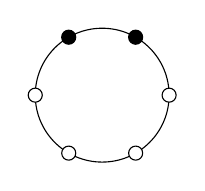
\begin{tikzpicture}[scale=0.85]
  \draw (0,0) circle (1.0);
  \foreach \a in {0,60,120,180,240,300}{
    \draw[fill=white] (\a:1) circle (0.105);
  }
  \foreach \a in {60,120}{
    \fill (\a:1) circle (0.105);
  }
\end{tikzpicture}
\end{center}

\[
D_6\times A\longrightarrow A,\qquad q=3.
\]

\bigskip
\noindent\underline{Benzen.}
% Schema moleculara urmeaza schita din manuscris: sase atomi C si sase H.
% Nu sunt adaugate legaturi duble, deoarece nu sunt desenate explicit in original.

\begin{center}
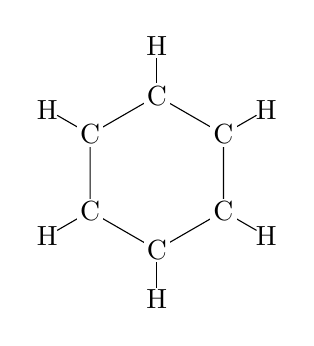
\begin{tikzpicture}[scale=0.85]
  \foreach \i in {0,...,5}{
    \pgfmathsetmacro{\ang}{90-60*\i}
    \coordinate (C\i) at (\ang:1.15);
    \draw (\ang:1.15) -- (\ang:1.72);
    \node[fill=white,inner sep=1.1pt] at (\ang:1.15) {$\mathrm{C}$};
    \node at (\ang:1.89) {$\mathrm{H}$};
  }
  \draw (C0)--(C1)--(C2)--(C3)--(C4)--(C5)--cycle;
  % Refacem etichetele C deasupra laturilor, pentru claritate.
  \foreach \i in {0,...,5}{
    \pgfmathsetmacro{\ang}{90-60*\i}
    \node[fill=white,inner sep=1.1pt] at (\ang:1.15) {$\mathrm{C}$};
  }
\end{tikzpicture}
\end{center}
.
% Fara preambul si fara schimbare fortata de pagina.
% Se pastreaza ordinea manuscrisului; comentariile marcheaza observatii editoriale.

\subsection*{Curs 11 - Pagina 4}

\noindent Fie $b\in G$. Atunci:
\[
by=y\iff b\in\operatorname{Stab}_G(y)
\iff bax=ax.
\]
\[
\iff a^{-1}bax=x
\iff a^{-1}ba\in\operatorname{Stab}_G(x)
\iff b\in a\operatorname{Stab}_G(x)a^{-1}.
\]

\bigskip
\noindent $A=\operatorname{orb}(z_1)\cup\cdots\cup
\operatorname{orb}(z_q)$ \quad (reuniune disjunctă).

\bigskip
\noindent $G=\{a_1,a_2,\ldots,a_m\}$, \quad $a_1=e$;
\qquad $A=\{x_1,\ldots,x_n\}$.

\medskip
\noindent Definim:
\[
\varepsilon_{ij}\overset{\mathrm{def}}{=}
\begin{cases}
1, & a_i x_j=x_j,\\
0, & a_i x_j\neq x_j,
\end{cases}
\quad (\forall)\ i=\overline{1,m},\quad
(\forall)\ j=\overline{1,n}.
\]

\noindent $\Rightarrow$ o matrice
$\bigl(\varepsilon_{ij}\bigr)_{\substack{i=\overline{1,m}\\j=\overline{1,n}}}$.

\bigskip
\noindent $S=\{(a_i,x_j)\in G\times A\mid a_i x_j=x_j\}$.

\noindent $|S|=\operatorname{nr.}(\varepsilon_{ij}=1)$.
\[
|S|=\sum_{i=1}^{m}\sum_{j=1}^{n}\varepsilon_{ij}.
\]

\noindent Pentru $i$ fixat:
\[
|\operatorname{Fix}a_i|=\sum_{j=1}^{n}\varepsilon_{ij}.
\]
% In manuscris, argumentul din "Fix" seamana pe alocuri cu x_i.
% Contextul indicilor (a_i in G) conduce la lectura a_i; de verificat.

\[
\Rightarrow\quad |S|=\sum_{i=1}^{m}|\operatorname{Fix}a_i|.
\]

\[
\begin{aligned}
|S|
&=\sum_{i=1}^{m}\sum_{j=1}^{n}\varepsilon_{ij}
 =\sum_{j=1}^{n}|\operatorname{Stab}_G(x_j)|\\[3pt]
&=\sum_{k=1}^{q}\left(
\sum_{\substack{x_j\in\operatorname{orb}(z_k)\\x_j\sim_G z_k}}
|\operatorname{Stab}_G(x_j)|\right)
 =q|G|.
\end{aligned}
\]

\bigskip
\noindent\underline{Brățară cu 6 pietre.}
% In desen se vad sase pietre, dintre care doua alaturate sunt umplute.
% Manuscrisul nu defineste explicit multimea A a colorarilor/configuratiilor.

\begin{center}
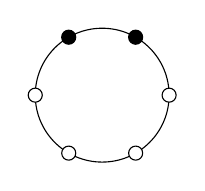
\begin{tikzpicture}[scale=0.85]
  \draw (0,0) circle (1.0);
  \foreach \a in {0,60,120,180,240,300}{
    \draw[fill=white] (\a:1) circle (0.105);
  }
  \foreach \a in {60,120}{
    \fill (\a:1) circle (0.105);
  }
\end{tikzpicture}
\end{center}

\[
D_6\times A\longrightarrow A,\qquad q=3.
\]

\bigskip
\noindent\underline{Benzen.}
% Schema moleculara urmeaza schita din manuscris: sase atomi C si sase H.
% Nu sunt adaugate legaturi duble, deoarece nu sunt desenate explicit in original.

\begin{center}
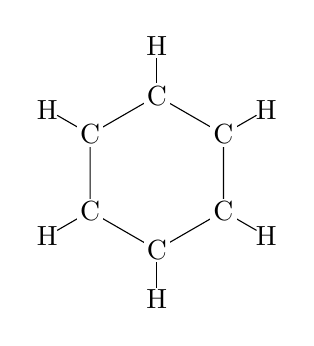
\begin{tikzpicture}[scale=0.85]
  \foreach \i in {0,...,5}{
    \pgfmathsetmacro{\ang}{90-60*\i}
    \coordinate (C\i) at (\ang:1.15);
    \draw (\ang:1.15) -- (\ang:1.72);
    \node[fill=white,inner sep=1.1pt] at (\ang:1.15) {$\mathrm{C}$};
    \node at (\ang:1.89) {$\mathrm{H}$};
  }
  \draw (C0)--(C1)--(C2)--(C3)--(C4)--(C5)--cycle;
  % Refacem etichetele C deasupra laturilor, pentru claritate.
  \foreach \i in {0,...,5}{
    \pgfmathsetmacro{\ang}{90-60*\i}
    \node[fill=white,inner sep=1.1pt] at (\ang:1.15) {$\mathrm{C}$};
  }
\end{tikzpicture}
\end{center}
.
% Fara preambul si fara schimbare fortata de pagina.
% Se pastreaza ordinea manuscrisului; comentariile marcheaza observatii editoriale.

\subsection*{Curs 11 - Pagina 4}

\noindent Fie $b\in G$. Atunci:
\[
by=y\iff b\in\operatorname{Stab}_G(y)
\iff bax=ax.
\]
\[
\iff a^{-1}bax=x
\iff a^{-1}ba\in\operatorname{Stab}_G(x)
\iff b\in a\operatorname{Stab}_G(x)a^{-1}.
\]

\bigskip
\noindent $A=\operatorname{orb}(z_1)\cup\cdots\cup
\operatorname{orb}(z_q)$ \quad (reuniune disjunctă).

\bigskip
\noindent $G=\{a_1,a_2,\ldots,a_m\}$, \quad $a_1=e$;
\qquad $A=\{x_1,\ldots,x_n\}$.

\medskip
\noindent Definim:
\[
\varepsilon_{ij}\overset{\mathrm{def}}{=}
\begin{cases}
1, & a_i x_j=x_j,\\
0, & a_i x_j\neq x_j,
\end{cases}
\quad (\forall)\ i=\overline{1,m},\quad
(\forall)\ j=\overline{1,n}.
\]

\noindent $\Rightarrow$ o matrice
$\bigl(\varepsilon_{ij}\bigr)_{\substack{i=\overline{1,m}\\j=\overline{1,n}}}$.

\bigskip
\noindent $S=\{(a_i,x_j)\in G\times A\mid a_i x_j=x_j\}$.

\noindent $|S|=\operatorname{nr.}(\varepsilon_{ij}=1)$.
\[
|S|=\sum_{i=1}^{m}\sum_{j=1}^{n}\varepsilon_{ij}.
\]

\noindent Pentru $i$ fixat:
\[
|\operatorname{Fix}a_i|=\sum_{j=1}^{n}\varepsilon_{ij}.
\]
% In manuscris, argumentul din "Fix" seamana pe alocuri cu x_i.
% Contextul indicilor (a_i in G) conduce la lectura a_i; de verificat.

\[
\Rightarrow\quad |S|=\sum_{i=1}^{m}|\operatorname{Fix}a_i|.
\]

\[
\begin{aligned}
|S|
&=\sum_{i=1}^{m}\sum_{j=1}^{n}\varepsilon_{ij}
 =\sum_{j=1}^{n}|\operatorname{Stab}_G(x_j)|\\[3pt]
&=\sum_{k=1}^{q}\left(
\sum_{\substack{x_j\in\operatorname{orb}(z_k)\\x_j\sim_G z_k}}
|\operatorname{Stab}_G(x_j)|\right)
 =q|G|.
\end{aligned}
\]

\bigskip
\noindent\underline{Brățară cu 6 pietre.}
% In desen se vad sase pietre, dintre care doua alaturate sunt umplute.
% Manuscrisul nu defineste explicit multimea A a colorarilor/configuratiilor.

\begin{center}
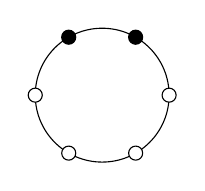
\begin{tikzpicture}[scale=0.85]
  \draw (0,0) circle (1.0);
  \foreach \a in {0,60,120,180,240,300}{
    \draw[fill=white] (\a:1) circle (0.105);
  }
  \foreach \a in {60,120}{
    \fill (\a:1) circle (0.105);
  }
\end{tikzpicture}
\end{center}

\[
D_6\times A\longrightarrow A,\qquad q=3.
\]

\bigskip
\noindent\underline{Benzen.}
% Schema moleculara urmeaza schita din manuscris: sase atomi C si sase H.
% Nu sunt adaugate legaturi duble, deoarece nu sunt desenate explicit in original.

\begin{center}
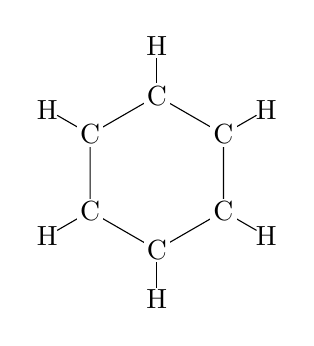
\begin{tikzpicture}[scale=0.85]
  \foreach \i in {0,...,5}{
    \pgfmathsetmacro{\ang}{90-60*\i}
    \coordinate (C\i) at (\ang:1.15);
    \draw (\ang:1.15) -- (\ang:1.72);
    \node[fill=white,inner sep=1.1pt] at (\ang:1.15) {$\mathrm{C}$};
    \node at (\ang:1.89) {$\mathrm{H}$};
  }
  \draw (C0)--(C1)--(C2)--(C3)--(C4)--(C5)--cycle;
  % Refacem etichetele C deasupra laturilor, pentru claritate.
  \foreach \i in {0,...,5}{
    \pgfmathsetmacro{\ang}{90-60*\i}
    \node[fill=white,inner sep=1.1pt] at (\ang:1.15) {$\mathrm{C}$};
  }
\end{tikzpicture}
\end{center}
.
% Fara preambul si fara schimbare fortata de pagina.
% Se pastreaza ordinea manuscrisului; comentariile marcheaza observatii editoriale.

\subsection*{Curs 11 - Pagina 4}

\noindent Fie $b\in G$. Atunci:
\[
by=y\iff b\in\operatorname{Stab}_G(y)
\iff bax=ax.
\]
\[
\iff a^{-1}bax=x
\iff a^{-1}ba\in\operatorname{Stab}_G(x)
\iff b\in a\operatorname{Stab}_G(x)a^{-1}.
\]

\bigskip
\noindent $A=\operatorname{orb}(z_1)\cup\cdots\cup
\operatorname{orb}(z_q)$ \quad (reuniune disjunctă).

\bigskip
\noindent $G=\{a_1,a_2,\ldots,a_m\}$, \quad $a_1=e$;
\qquad $A=\{x_1,\ldots,x_n\}$.

\medskip
\noindent Definim:
\[
\varepsilon_{ij}\overset{\mathrm{def}}{=}
\begin{cases}
1, & a_i x_j=x_j,\\
0, & a_i x_j\neq x_j,
\end{cases}
\quad (\forall)\ i=\overline{1,m},\quad
(\forall)\ j=\overline{1,n}.
\]

\noindent $\Rightarrow$ o matrice
$\bigl(\varepsilon_{ij}\bigr)_{\substack{i=\overline{1,m}\\j=\overline{1,n}}}$.

\bigskip
\noindent $S=\{(a_i,x_j)\in G\times A\mid a_i x_j=x_j\}$.

\noindent $|S|=\operatorname{nr.}(\varepsilon_{ij}=1)$.
\[
|S|=\sum_{i=1}^{m}\sum_{j=1}^{n}\varepsilon_{ij}.
\]

\noindent Pentru $i$ fixat:
\[
|\operatorname{Fix}a_i|=\sum_{j=1}^{n}\varepsilon_{ij}.
\]
% In manuscris, argumentul din "Fix" seamana pe alocuri cu x_i.
% Contextul indicilor (a_i in G) conduce la lectura a_i; de verificat.

\[
\Rightarrow\quad |S|=\sum_{i=1}^{m}|\operatorname{Fix}a_i|.
\]

\[
\begin{aligned}
|S|
&=\sum_{i=1}^{m}\sum_{j=1}^{n}\varepsilon_{ij}
 =\sum_{j=1}^{n}|\operatorname{Stab}_G(x_j)|\\[3pt]
&=\sum_{k=1}^{q}\left(
\sum_{\substack{x_j\in\operatorname{orb}(z_k)\\x_j\sim_G z_k}}
|\operatorname{Stab}_G(x_j)|\right)
 =q|G|.
\end{aligned}
\]

\bigskip
\noindent\underline{Brățară cu 6 pietre.}
% In desen se vad sase pietre, dintre care doua alaturate sunt umplute.
% Manuscrisul nu defineste explicit multimea A a colorarilor/configuratiilor.

\begin{center}
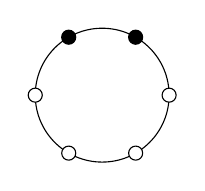
\begin{tikzpicture}[scale=0.85]
  \draw (0,0) circle (1.0);
  \foreach \a in {0,60,120,180,240,300}{
    \draw[fill=white] (\a:1) circle (0.105);
  }
  \foreach \a in {60,120}{
    \fill (\a:1) circle (0.105);
  }
\end{tikzpicture}
\end{center}

\[
D_6\times A\longrightarrow A,\qquad q=3.
\]

\bigskip
\noindent\underline{Benzen.}
% Schema moleculara urmeaza schita din manuscris: sase atomi C si sase H.
% Nu sunt adaugate legaturi duble, deoarece nu sunt desenate explicit in original.

\begin{center}
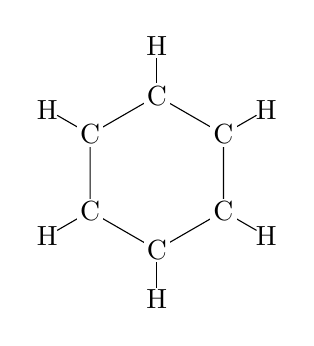
\begin{tikzpicture}[scale=0.85]
  \foreach \i in {0,...,5}{
    \pgfmathsetmacro{\ang}{90-60*\i}
    \coordinate (C\i) at (\ang:1.15);
    \draw (\ang:1.15) -- (\ang:1.72);
    \node[fill=white,inner sep=1.1pt] at (\ang:1.15) {$\mathrm{C}$};
    \node at (\ang:1.89) {$\mathrm{H}$};
  }
  \draw (C0)--(C1)--(C2)--(C3)--(C4)--(C5)--cycle;
  % Refacem etichetele C deasupra laturilor, pentru claritate.
  \foreach \i in {0,...,5}{
    \pgfmathsetmacro{\ang}{90-60*\i}
    \node[fill=white,inner sep=1.1pt] at (\ang:1.15) {$\mathrm{C}$};
  }
\end{tikzpicture}
\end{center}
